\documentclass[11pt]{article}

\usepackage[margin=1in]{geometry}
\usepackage{amsmath,amssymb,amsthm,mathtools}
\usepackage{graphicx}
\usepackage{microtype}
\usepackage{enumitem}
\usepackage{xcolor}
\usepackage[colorlinks=true,linkcolor=blue!55!black,citecolor=blue!55!black,urlcolor=blue!65!black]{hyperref}

\newtheorem{theorem}{Theorem}
\newtheorem{corollary}[theorem]{Corollary}
\newtheorem{lemma}[theorem]{Lemma}
\newtheorem{remark}[theorem]{Remark}

\newcommand{\R}{\mathbb R}
\newcommand{\ext}{\operatorname{ext}}
\newcommand{\spr}{\operatorname{spr}}
\newcommand{\ov}{\operatorname{ov}}

\title{An extreme-boundary characterization of non-SPR\\
isometric embeddings into $C(K)$}
\author{Candidate full solution to Question 6.6 of arXiv:2210.05114}
\date{19 July 2026}

\begin{document}
\maketitle

\begin{center}
\fbox{\parbox{0.91\textwidth}{
\textbf{Status: candidate full solution; human review required.}
For real Banach spaces, this packet gives an intrinsic necessary-and-sufficient
criterion for the existence of an isometric embedding into some $C(K)$ whose
range fails stable phase retrieval.  It also identifies the sharp worst-case
SPR constant over all isometric $C(K)$-representations.
}}
\end{center}

\section{Source and exact question}

The source is D. Freeman, T. Oikhberg, B. Pineau, and M. A. Taylor,
\emph{Stable phase retrieval in function spaces}, arXiv:2210.05114v1,
submitted 11 October 2022 and subsequently published in
\emph{Mathematische Annalen} 390 (2024) \cite{FOPT}.  Unless explicitly
stated otherwise, the source works over the real field.  Question 6.6 is on
page 48 of the arXiv PDF:

\begin{figure}[ht]
  \centering
  
\includegraphics[width=\textwidth]{figures/open_problem_crop.png}
  \caption{Question 6.6, rendered from page 48 of the source PDF.}
\end{figure}

\paragraph{Transcription.}
``Which Banach spaces $E$ isometrically embed into $C(K)$ in a non-SPR way?''

Immediately after the question, the source proves a three-dimensional example
for which every isometric $C(K)$-embedding is SPR.  Its Lemma 6.8 supplies the
one-sided extreme-point estimate that motivates the answer below:

\begin{figure}[ht]
  \centering
  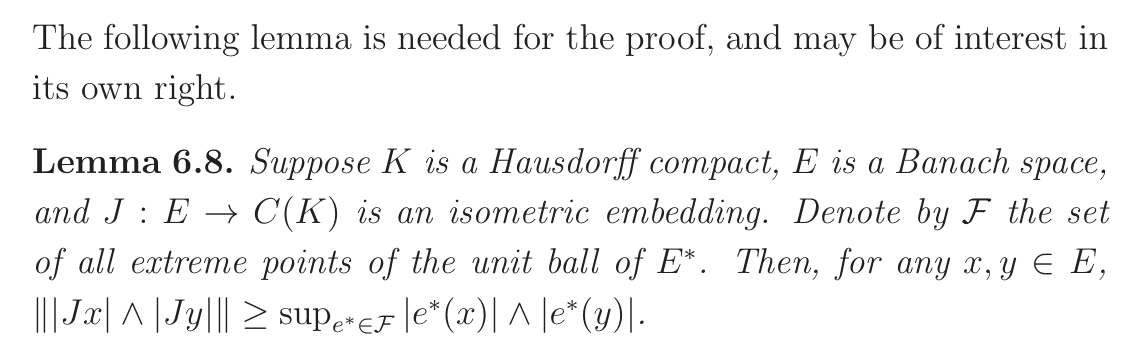
\includegraphics[width=\textwidth]{figures/source_lemma_6_8.png}
  \caption{The statement of source Lemma 6.8, rendered from page 48.}
\end{figure}

\section{Definitions}

Throughout, $E$ is a nonzero real Banach space.  If
$J:E\to C(K)$ is a linear isometric embedding, define its \emph{overlap
constant}
\[
 \ov(J):=\inf_{x,y\in S_E}
 \bigl\|\,|Jx|\wedge|Jy|\,\bigr\|_\infty.
\]
The range $J(E)$ does $C$-stable phase retrieval ($C$-SPR) when
\[
 \min\{\|Jx-Jy\|_\infty,\|Jx+Jy\|_\infty\}
 \leq C\bigl\|\,|Jx|-|Jy|\,\bigr\|_\infty
 \qquad(x,y\in E).
\]
Write $\spr(J)$ for the optimal such constant, with $\spr(J)=\infty$ if
the range is not SPR.

Let $\mathcal E_E=\ext B_{E^*}$ and introduce the intrinsic
\emph{extreme-boundary overlap}
\begin{equation}\label{eq:Delta}
 \Delta(E):=
 \inf_{x,y\in S_E}\ \sup_{e^*\in\mathcal E_E}
 \bigl(|e^*(x)|\wedge|e^*(y)|\bigr).
\end{equation}
This number depends only on the isometric Banach-space structure of $E$; it
does not refer to an ambient function space.

\section{Proof Intuition}

Every isometric representation $J:E\to C(K)$ must display every extreme
functional of $B_{E^*}$ as a signed point evaluation.  Therefore the overlap
of $Jx$ and $Jy$ can never be smaller than the simultaneous values forced by
those extreme functionals.  This is the source's Lemma 6.8.

The missing converse is obtained by using the smallest canonical compactum
that contains exactly this information:
\[
 K_E=\overline{\ext B_{E^*}}^{,w^*}.
\]
Krein--Milman makes the evaluation map $x\mapsto(e^*\mapsto e^*(x))$ an
isometry into $C(K_E)$, while weak-star continuity shows that its overlap is
\emph{exactly} the extreme-boundary quantity in \eqref{eq:Delta}.  Finally, a
real lattice identity converts overlap into the optimal SPR constant with no
loss.  Hence $\Delta(E)=0$ is precisely the requested criterion for a non-SPR
isometric embedding.

\section{Full characterization}

\begin{theorem}[Sharp extreme-boundary criterion]\label{thm:main}
Let $E$ be a nonzero real Banach space and define $\Delta(E)$ by
\eqref{eq:Delta}.  Then:
\begin{enumerate}[label=\textup{(\roman*)}]
\item for every compact Hausdorff $K$ and every linear isometry
$J:E\to C(K)$,
\[
 \ov(J)\geq\Delta(E),
 \qquad
 \spr(J)\leq\frac{1}{\Delta(E)},
\]
with the convention $1/0=\infty$;
\item if
\[
 K_E=\overline{\ext B_{E^*}}^{w^*}
 \quad\text{and}\quad
 (J_E x)(e^*)=e^*(x),
\]
then $K_E$ is compact Hausdorff, $J_E:E\to C(K_E)$ is a linear isometry,
and
\[
 \ov(J_E)=\Delta(E),
 \qquad
 \spr(J_E)=\frac{1}{\Delta(E)}.
\]
\item consequently, the following are equivalent:
\begin{enumerate}[label=\textup{(\alph*)}]
\item $E$ admits a non-SPR linear isometric embedding into $C(K)$ for some
compact Hausdorff $K$;
\item the canonical embedding $J_E:E\to C(K_E)$ is non-SPR;
\item $\Delta(E)=0$.
\end{enumerate}
Moreover,
\[
 \sup\{\spr(J):J:E\to C(K)\text{ a linear isometry},\ K\text{ compact}\}
 =\frac1{\Delta(E)}.
\]
\end{enumerate}
Thus $\Delta(E)=0$ is an intrinsic and sharp answer to Question 6.6.
\end{theorem}

\begin{proof}
We separate the proof into three exact ingredients.

\medskip
\noindent\textbf{1. Overlap and the optimal real SPR constant.}
For elements $u,v$ of a real vector lattice, the scalar identity applied by
lattice functional calculus is
\begin{equation}\label{eq:latticeidentity}
 \bigl|\,|u+v|-|u-v|\,\bigr|=2(|u|\wedge|v|).
\end{equation}
Let $F$ be any real normed subspace of a Banach lattice, and put
$d_F=\inf_{u,v\in S_F}\||u|\wedge|v|\|$.  If $u,v$ are nonzero and
$a=\|u\|\leq b=\|v\|$, monotonicity of the lattice infimum and lattice norm
gives
\begin{align*}
 \||u|\wedge|v|\|
 &=a\left\|\left|\frac ua\right|
      \wedge\frac ba\left|\frac vb\right|\right\|\\
 &\geq a\left\|\left|\frac ua\right|
      \wedge\left|\frac vb\right|\right\|
 \geq a d_F.
\end{align*}
Hence
\begin{equation}\label{eq:overlapineq}
 \min\{\|u\|,\|v\|\}
 \leq d_F^{-1}\||u|\wedge|v|\|.
\end{equation}
Conversely, substitute $f=u+v$ and $g=u-v$ in the SPR inequality.  Its
left side is $2\min\{\|u\|,\|v\|\}$, while by
\eqref{eq:latticeidentity} its modulus-difference term is
$2\||u|\wedge|v|\|$.  Thus no SPR constant smaller than $1/d_F$ is possible.
Applying \eqref{eq:overlapineq} to
$u=(f+g)/2$, $v=(f-g)/2$ proves the converse inequality.  Therefore
\begin{equation}\label{eq:opt}
 \text{the optimal real SPR constant of }F\text{ is exactly }1/d_F,
\end{equation}
again with value $\infty$ when $d_F=0$.  In particular,
$\spr(J)=1/\ov(J)$.

\medskip
\noindent\textbf{2. Every isometric embedding dominates the extreme
boundary.}
We recall and include the short proof of source Lemma 6.8 \cite[Lemma 6.8]{FOPT}.
Let $J:E\to C(K)$ be a linear isometry and fix
$e^*\in\ext B_{E^*}$.  Hahn--Banach gives a measure
$\mu\in M(K)=C(K)^*$ with
\[
 \|\mu\|=1,
 \qquad J^*\mu=e^*.
\]
The fibre
\[
 \mathcal F_{e^*}=\{\nu\in B_{M(K)}:J^*\nu=e^*\}
\]
is nonempty, weak-star compact, and convex, so it has an extreme point $\nu$.
If $\nu=(\nu_1+\nu_2)/2$ with $\nu_i\in B_{M(K)}$, then
\[
 e^*=\frac{J^*\nu_1+J^*\nu_2}{2}.
\]
Extremality of $e^*$ in $B_{E^*}$ forces
$J^*\nu_1=J^*\nu_2=e^*$; extremality of $\nu$ in the fibre then forces
$\nu_1=\nu_2=\nu$.  Thus $\nu$ is extreme in $B_{M(K)}$.  The extreme
points of the real measure ball are $\pm\delta_t$ for $t\in K$, so
$e^*=\pm J^*\delta_t$ for some $t$.  Consequently, for all $x,y\in E$,
\[
 \bigl\|\,|Jx|\wedge|Jy|\,\bigr\|_\infty
 \geq |e^*(x)|\wedge|e^*(y)|.
\]
Taking the supremum over $e^*$ and then the infimum over $x,y\in S_E$ gives
$\ov(J)\geq\Delta(E)$.  Formula \eqref{eq:opt} proves part (i).

\medskip
\noindent\textbf{3. The canonical extreme-boundary embedding attains the
bound.}
By Banach--Alaoglu and Krein--Milman \cite[Chapters 3--4]{Megginson},
$K_E=\overline{\ext B_{E^*}}^{w^*}$ is a nonempty compact Hausdorff space and
the extreme points norm $E$.  Therefore
\[
 \|J_E x\|_{C(K_E)}
 =\sup_{e^*\in K_E}|e^*(x)|
 =\sup_{e^*\in\ext B_{E^*}}|e^*(x)|
 =\|x\|,
\]
so $J_E$ is a linear isometry.  For fixed $x,y$, the function
\[
 e^*\longmapsto |e^*(x)|\wedge|e^*(y)|
\]
is weak-star continuous.  Its supremum over $K_E$ therefore equals its
supremum over the dense subset $\ext B_{E^*}$.  It follows that
\begin{align*}
 \ov(J_E)
 &=\inf_{x,y\in S_E}\sup_{e^*\in K_E}
       (|e^*(x)|\wedge|e^*(y)|)\\
 &=\inf_{x,y\in S_E}\sup_{e^*\in\ext B_{E^*}}
       (|e^*(x)|\wedge|e^*(y)|)
 =\Delta(E).
\end{align*}
Formula \eqref{eq:opt} now gives
$\spr(J_E)=1/\Delta(E)$.  The equivalences and the sharp supremum statement
follow immediately.
\end{proof}

\section{Concrete consequences}

\begin{corollary}[Finite-dimensional form]\label{cor:finite}
If $E$ is finite dimensional, then $E$ admits a non-SPR isometric embedding
into some $C(K)$ if and only if there exist $x,y\in S_E$ such that
\[
 \text{for every }e^*\in\ext B_{E^*},
 \qquad e^*(x)=0\quad\text{or}\quad e^*(y)=0.
\]
For a polyhedral space this is a finite vertex test on $B_{E^*}$.
\end{corollary}

\begin{proof}
In finite dimensions, $S_E\times S_E$ is compact.  The function
\[
 (x,y)\longmapsto\sup_{e^*\in K_E}
 (|e^*(x)|\wedge|e^*(y)|)
\]
is continuous because it is the maximum of a jointly continuous function over
the compact set $K_E$.  Hence the infimum defining $\Delta(E)$ is attained.
It is zero exactly under the displayed annihilation alternative, and
Theorem~\ref{thm:main} applies.
\end{proof}

For example, $E=\ell_\infty^2$ has $\Delta(E)=0$: take
$x=(1,0)$ and $y=(0,1)$, while the extreme points of $B_{E^*}=B_{\ell_1^2}$
are the signed coordinate functionals.  Thus the identity representation of
$\ell_\infty^2$ is non-SPR.  By contrast, the three-dimensional space in
source Proposition 6.7 satisfies $\Delta(E)\geq1/3$ by the calculation in that
proposition, so every isometric $C(K)$-embedding is at worst $3$-SPR.  These
examples illustrate that the criterion detects precisely the phenomenon that
uniform non-squareness alone does not classify.

\section{Verification notes}

The accompanying \texttt{verification.md} gives a separate adversarial audit.
The main checks are:
\begin{enumerate}[leftmargin=*]
\item the result is explicitly real-scalar, matching the source convention;
\item $K_E$ is weak-star compact even when $E$ is nonseparable, and the
evaluation functions are continuous;
\item Krein--Milman makes the extreme boundary norming, so the canonical map
is genuinely isometric;
\item taking weak-star closure does not change the relevant supremum because
the simultaneous-overlap function is continuous;
\item the real lattice identity gives the \emph{optimal} reciprocal constant,
not merely one implication;
\item the source's one-sided lemma applies to every isometric embedding, while
the canonical construction proves attainability and the missing converse.
\end{enumerate}
No computational experiment is used as proof.  The packet's only code renders
the two source crops from the copied source PDF.

\section{Scope, novelty check, and review recommendation}

\paragraph{Scope.}
The theorem fully answers Question 6.6 in the source's real-scalar setting by
an intrinsic isometric criterion.  It does not give a classification by
Banach-space isomorphism type, and it does not claim the analogous sharp
criterion for complex SPR, whose phase group is larger and whose overlap
condition is not sufficient.

\paragraph{Bounded novelty check.}
On 19 July 2026, the run's registry, solution, attempt, and proof-gap indexes
were searched for arXiv:2210.05114, Question 6.6, non-SPR isometric embeddings,
extreme points, and canonical boundary embeddings; no duplicate was found.
Exact-phrase web searches and author/title searches were also performed.  The
source paper and the later arXiv papers 2504.06693, 2512.08110, and 2512.08114
were checked in full text where relevant.  Those later papers treat complex
SPR or the distinct Cantor--Bendixson hierarchy Question 6.4; no statement
matching Theorem~\ref{thm:main} was located.  The source already contains the
one-sided Lemma 6.8, but it does not state the canonical attainability,
necessary-and-sufficient criterion, or optimal worst-case constant proved
here.  This was a bounded search and does not establish originality.

\paragraph{Human-review recommendation.}
Treat the packet as a likely valid candidate full answer to the exact real
Question 6.6.  The highest-value review issue is conceptual: decide whether an
intrinsic sharp extreme-boundary criterion counts as the intended
``which spaces'' classification, or whether the question sought only a
description in pre-existing geometric classes.  Mathematically, reviewers
should audit the fibre-extreme-point argument and the claim that the canonical
boundary embedding attains the universal lower bound.

\begin{thebibliography}{9}
\bibitem{FOPT}
D. Freeman, T. Oikhberg, B. Pineau, and M. A. Taylor,
\emph{Stable phase retrieval in function spaces},
arXiv:2210.05114v1 (2022); \emph{Math. Ann.} 390 (2024),
\url{https://arxiv.org/abs/2210.05114}.

\bibitem{Megginson}
R. E. Megginson,
\emph{An Introduction to Banach Space Theory},
Graduate Texts in Mathematics 183, Springer, 1998.
\end{thebibliography}

\end{document}
